\chapter{Manuel Utilisateur}

\section{Application Android}

L'application Android permet à l'utilisateur de suivre son trajet sur une carte Google Maps et de faire une course contre un autre trajet.

Tout d'abord, lors du lancement de l'application, il faut se connecter avec son identifiant et son mot de passe pour arriver sur la carte. La navigation se fait avec trois onglets. Le premier onglet correspond à la carte où l'on peut voir sa position et de plus le trajet que l'on est en train de faire durant une course.

Le deuxième onglet montre toutes les catégories que l'utilisateur a créé et il peut en créer de nouvelles. Dans ces catégories, l'utilisateur peut choisir le trajet contre lequel il veut faire la course.

Et enfin le troisième onglet correspond à la page des options où l'utilisateur peut par exemple changer le thème de la carte en plus sombre (une actualisation de la position sur la carte est nécessaire pour que le thème change) ou encore se déconnecter.

\section{Site web}

Le site web a une interface très simple d'utilisation. La page d'accueil décrit très simplement le but de l'application GhostRun.

En haut à gauche de la page d'accueil \autoref{fig:80-accueil}, nous avons le bouton Espace membres, qui n'est disponibles que si l'utilisateur s'est connecté. Il peut le faire avec le bouton Connexion en haut à droite. Les identifiants de l'utilisateur sont les mêmes que ceux sur l'application. Si un utilisateur essaye d'accéder à l'une de ces pages sans être connecté, il sera redirigé sur la page de connexion.

\begin{figure}[H]
    \centering
    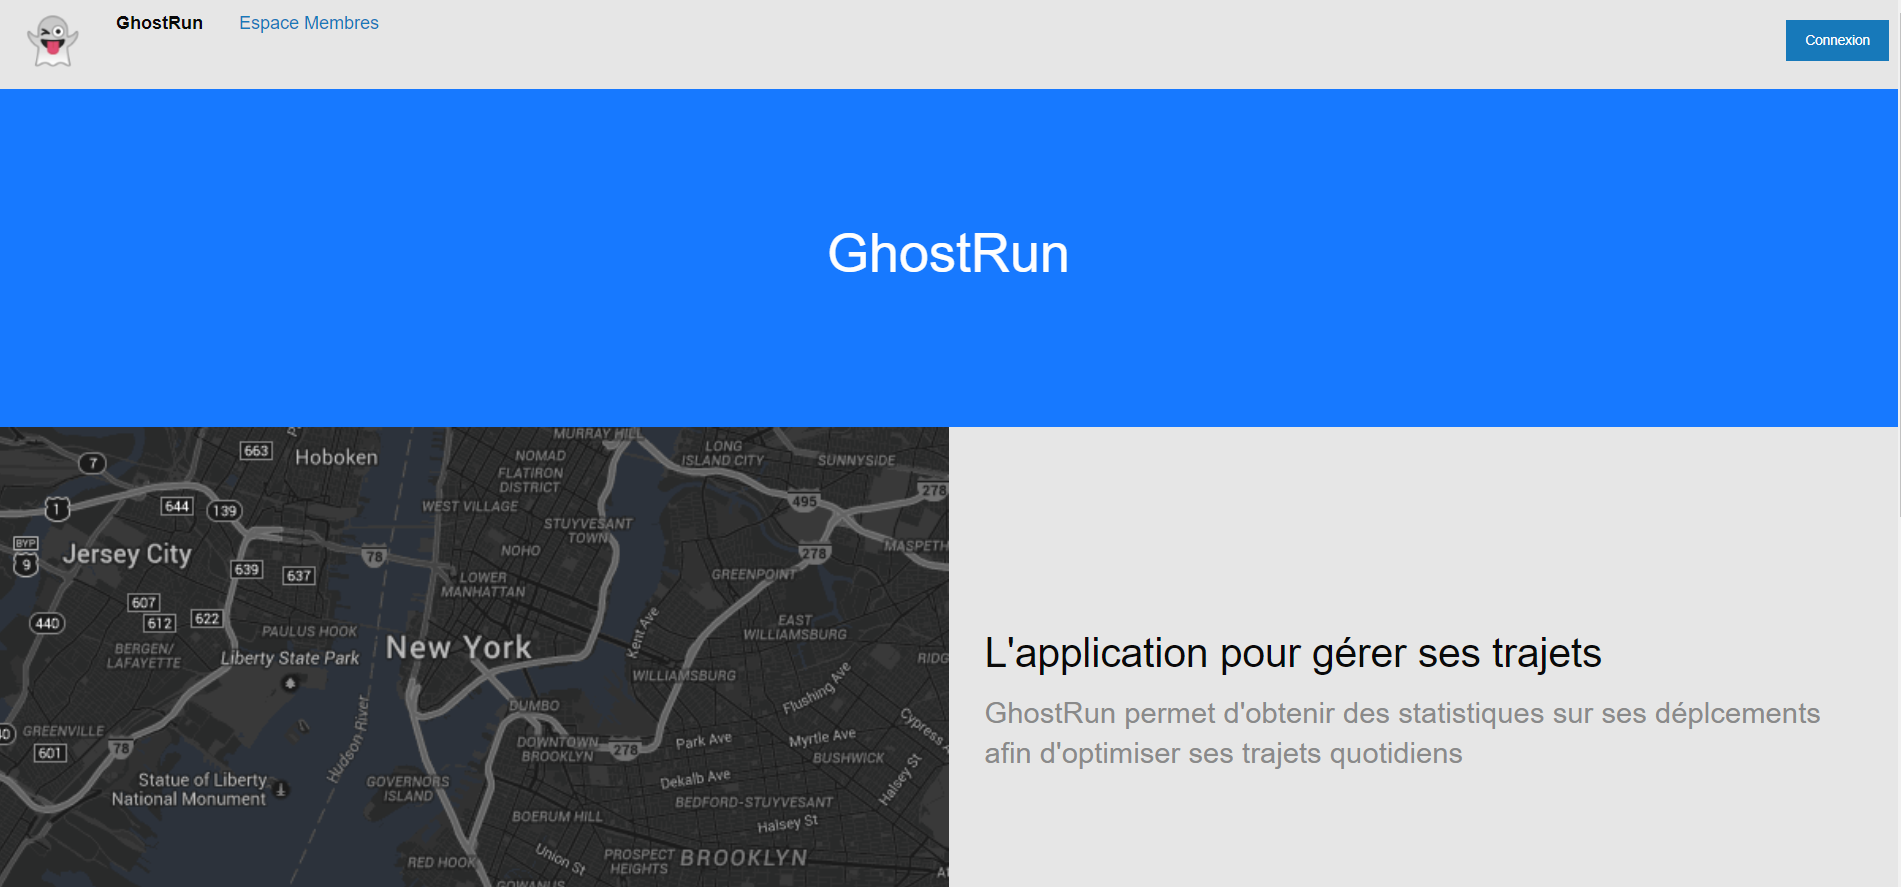
\includegraphics[keepaspectratio, width=2\textwidth/2, height=2\textheight/5]{ima/accueil}
    \caption{Page d'accueil du site web GhostRun}
    \label{fig:80-accueil}
\end{figure}

Après s'être connecté, l'utilisateur a donc accès à son espace membres où il peut voir tous les trajets qu'il a réalisé dans chacune de ses catégories (\autoref{fig:80-espace}). En cliquant sur l'un des trajets, il peut voir plusieurs statistiques sur ce trajet (comme la distance parcourue, sa vitesse moyenne, la durée du trajet, ou encore un graphique du dénivelé). Il peut aussi bien évidemment consulter l'itinéraire parcouru sur la carte à gauche de la page ou encore supprimer le trajet. Tout ceci peut lui permettre de faire son choix sur quel trajet il souhaite réaliser une course (\autoref{fig:80-stat}).

\begin{figure}[H]
    \centering
    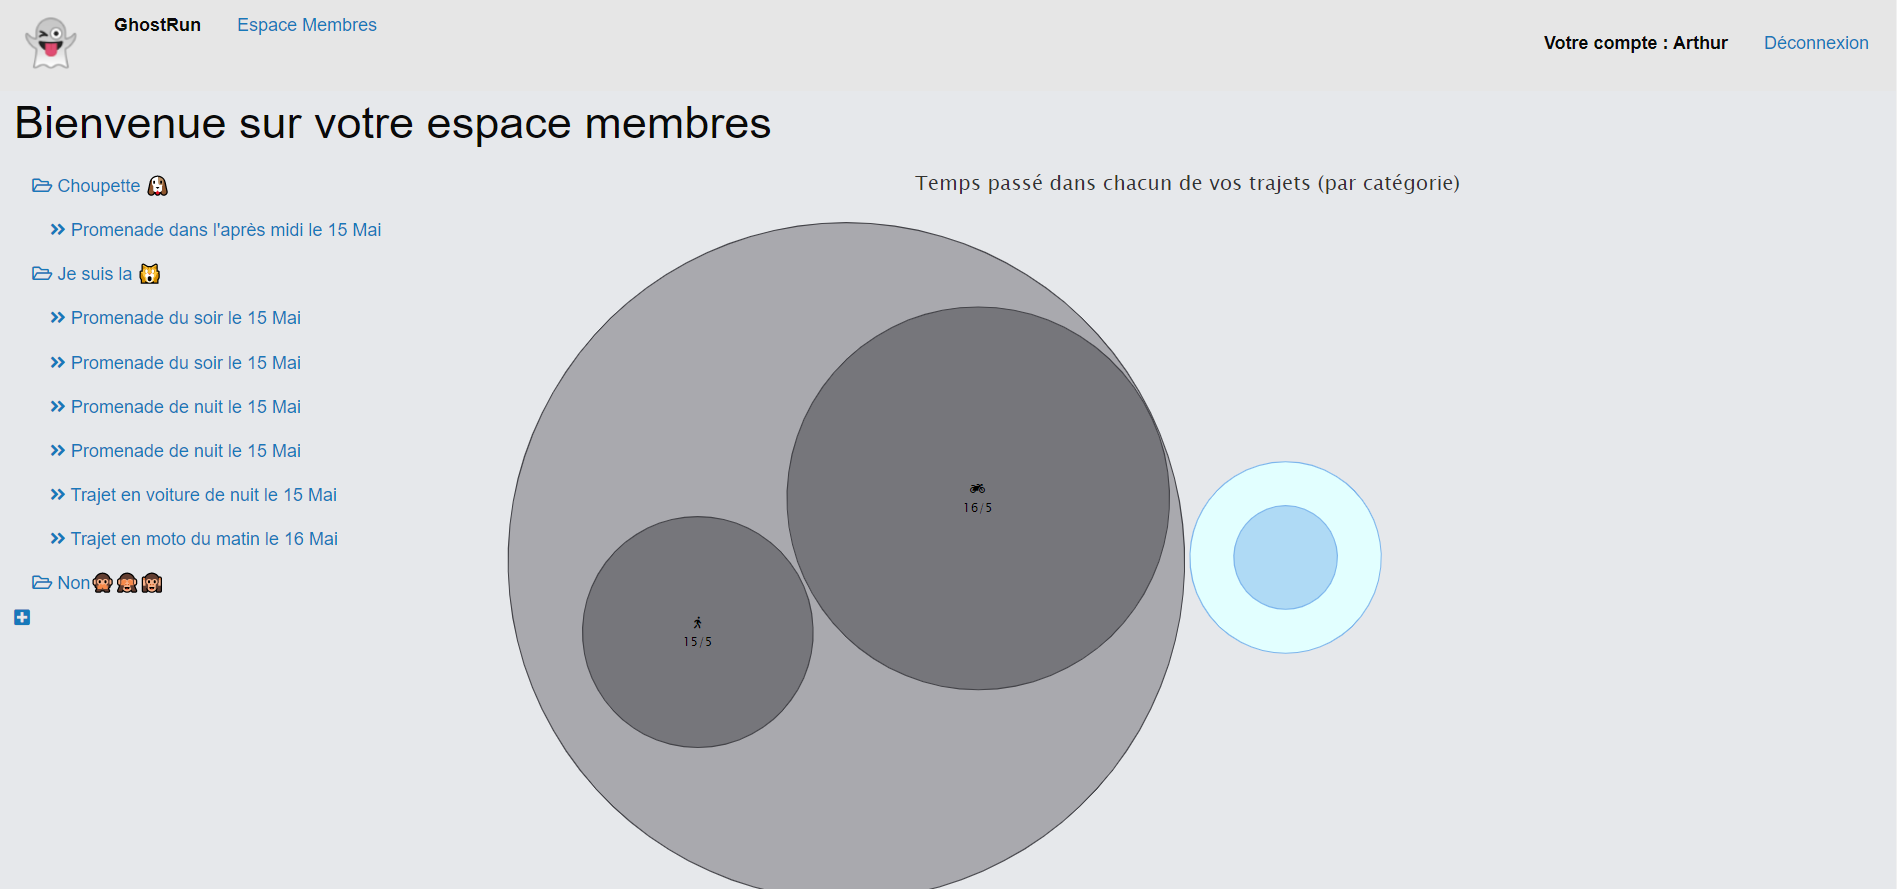
\includegraphics[keepaspectratio, width=2\textwidth/2, height=2\textheight/5]{ima/espace}
    \caption{Espace membres du site web GhostRun}
    \label{fig:80-espace}
\end{figure}

\begin{figure}[H]
    \centering
    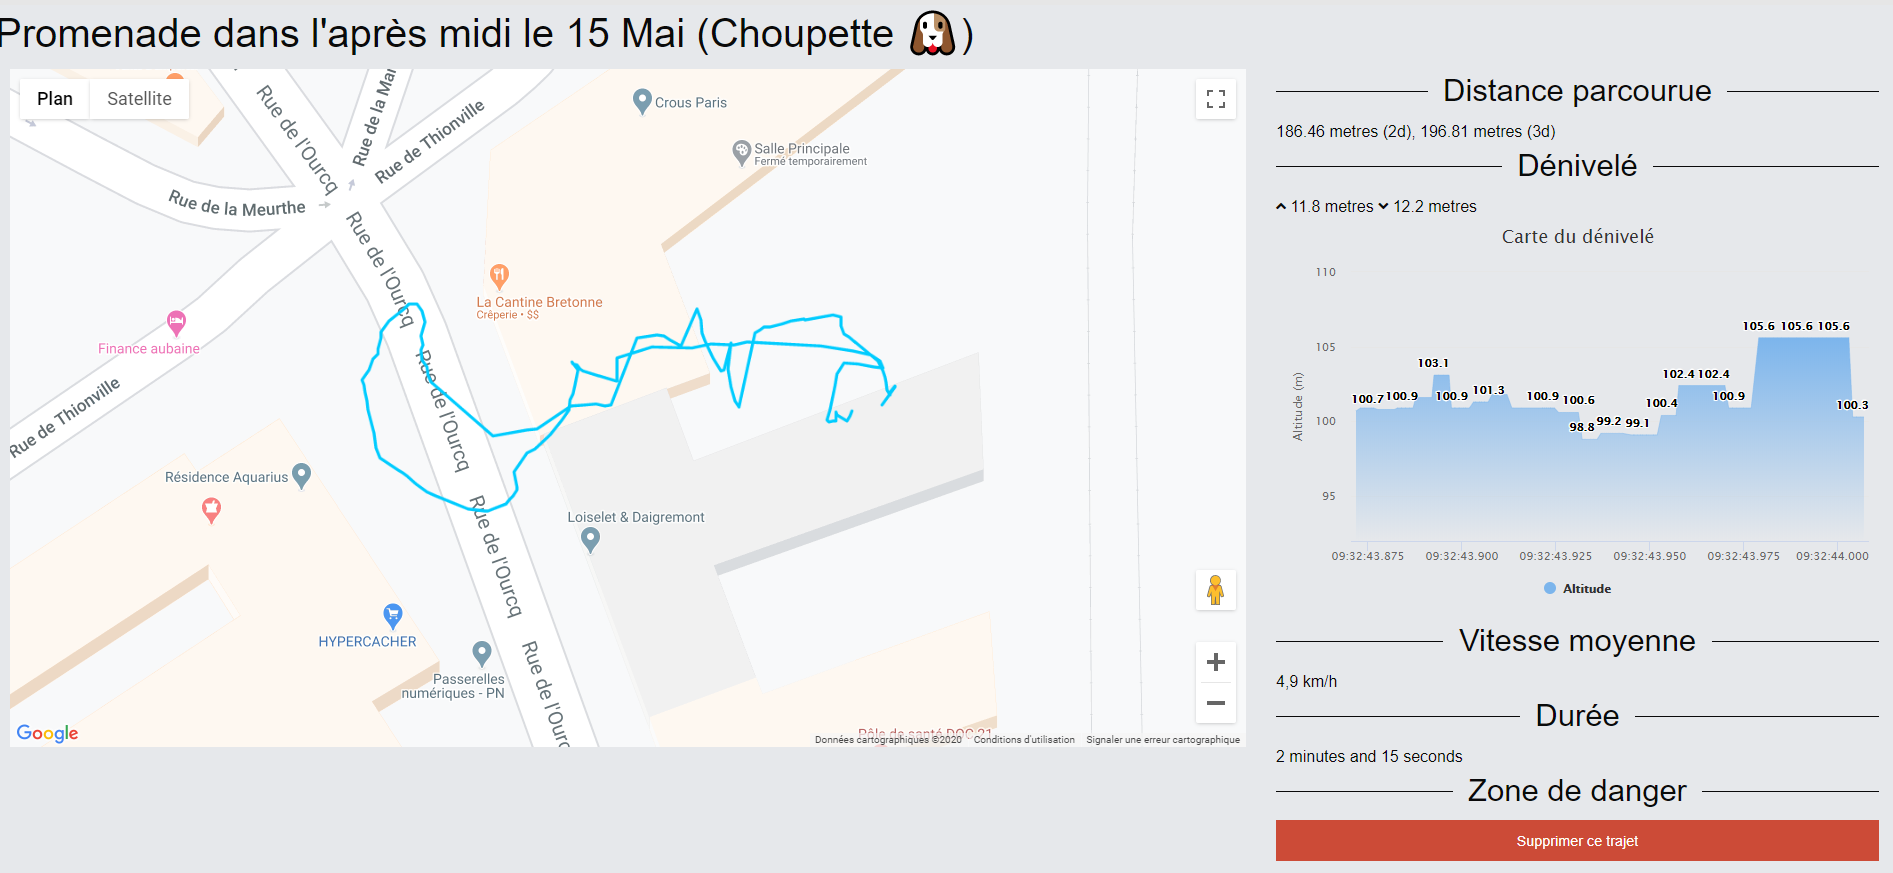
\includegraphics[keepaspectratio, width=2\textwidth/2, height=2\textheight/5]{ima/stat}
    \caption{Statistiques d'un trajet}
    \label{fig:80-stat}
\end{figure}


\section{Interface administrateur}

L'interface administrateur permet aux administrateur de consulter la base de données depuis une interface plus agréable que des commandes SQL. Elle est générée dynamiquement en fonction des tables définies. Elle permet d'ajouter, de supprimer ou de modifier les données concernant n'importe quel trajet ou catégorie de n'importe quel utilisateur. Son accès est réservé aux comptes disposant de l'attribut "super-utilisateur".

\begin{figure}[H]
    \centering
    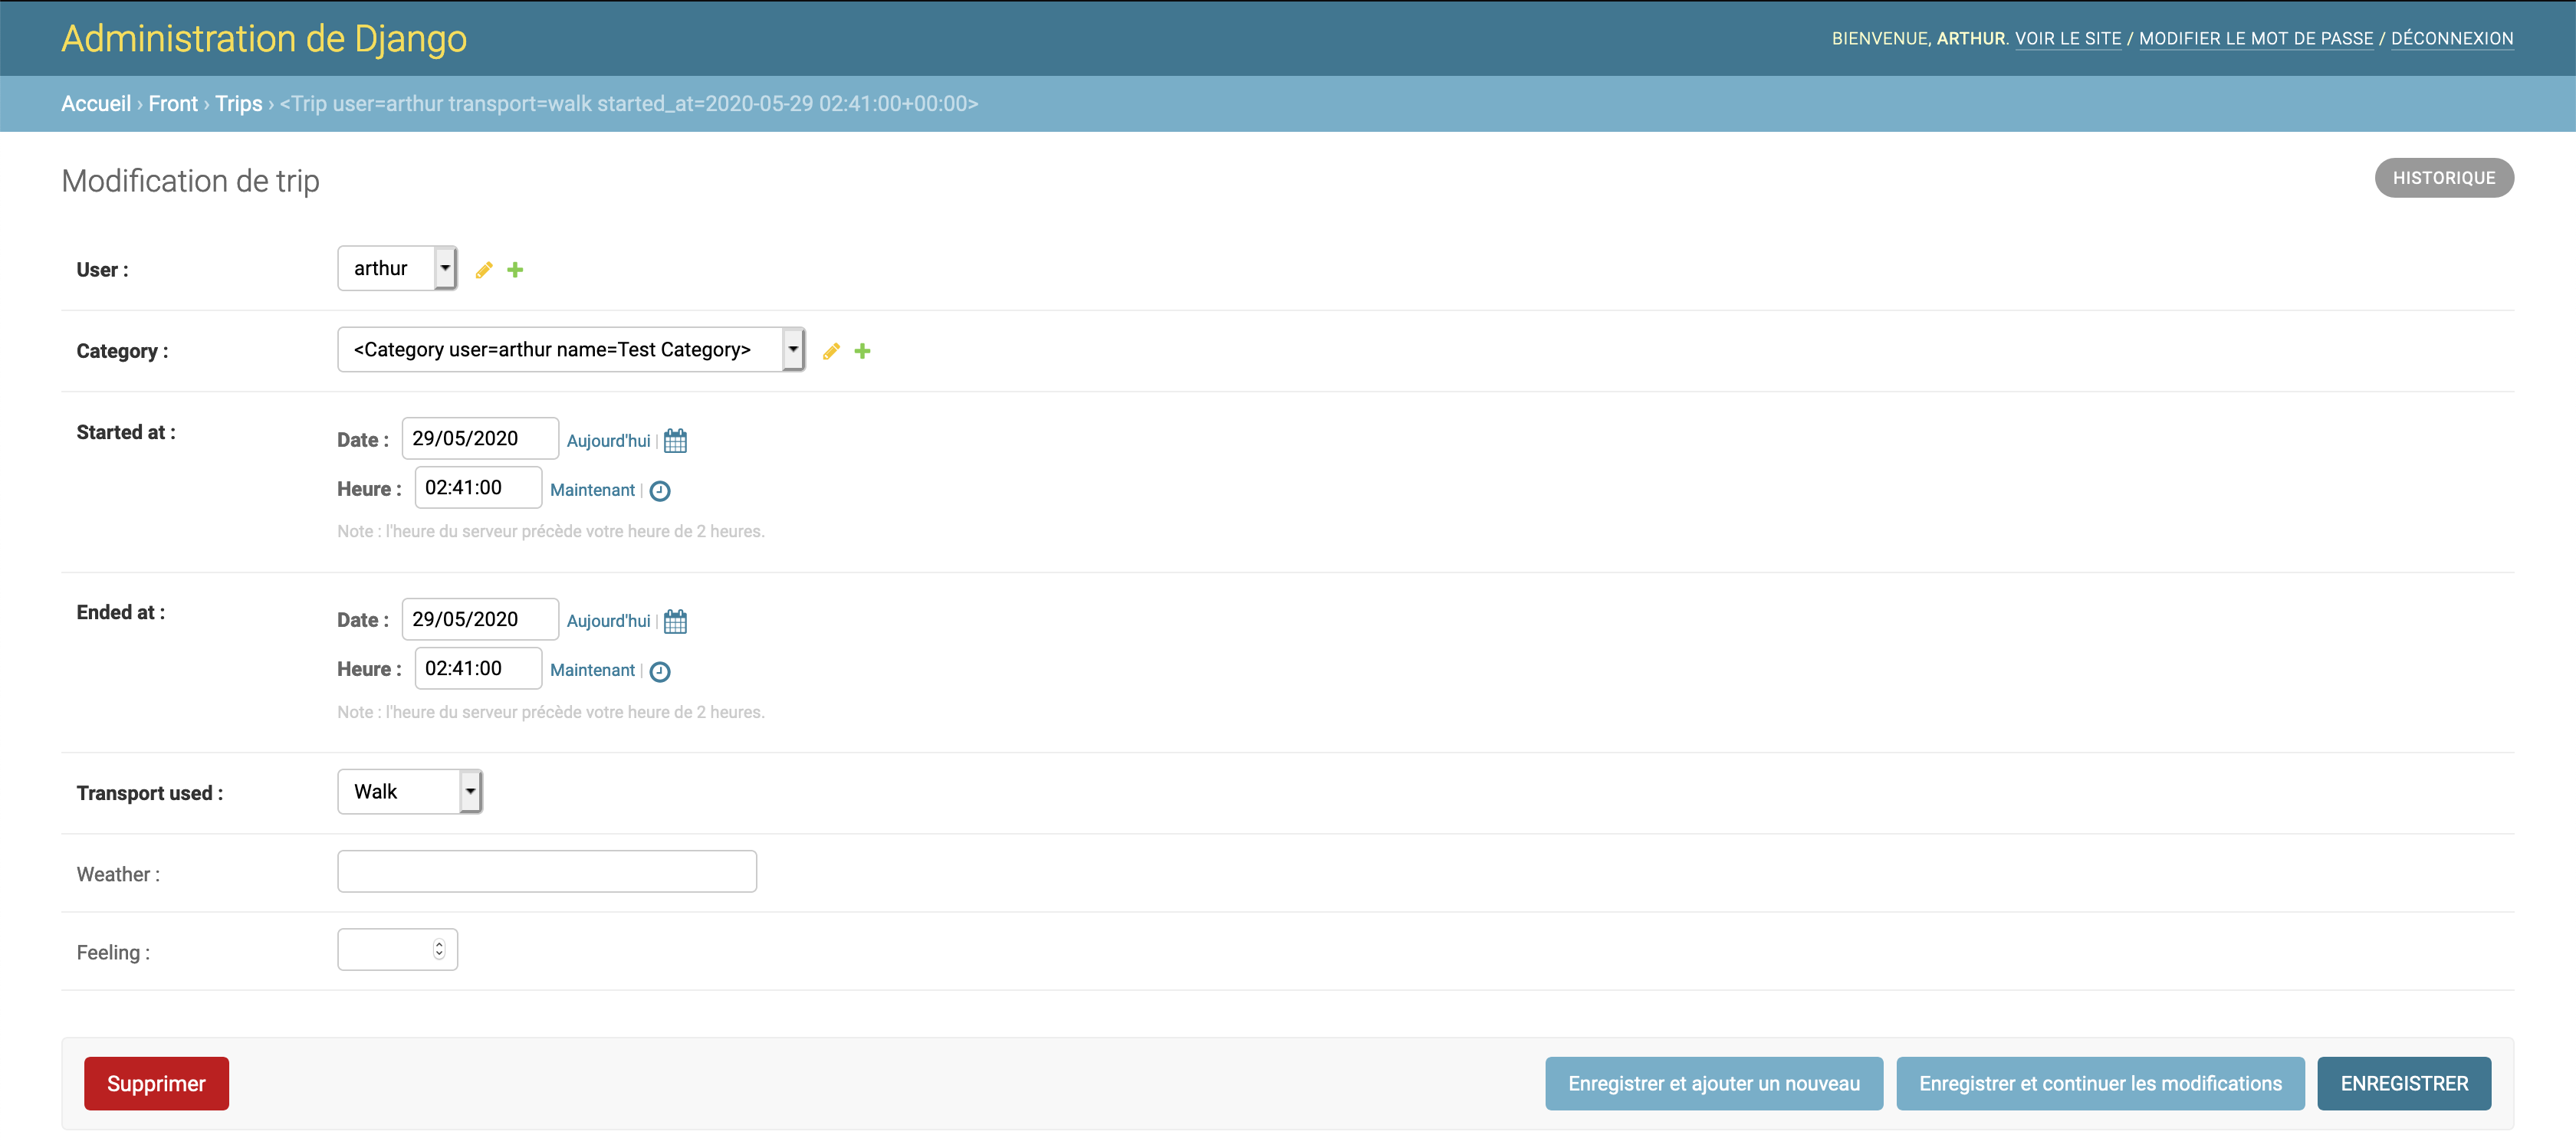
\includegraphics[keepaspectratio, width=2\textwidth/2, height=2\textheight/5]{ima/interface-admin}
    \caption{L'interface administrateur en images.}
    \label{fig:80-interface-administrateur}
\end{figure}


\section{API}

L'\gls{API} est une interface permettant à des services externes de se connecter au site web et de lui communiquer des données, ou d'en récupérer. Un utilisateur souhaitant utiliser l'\gls{API}, par exemple à travers l'application téléphone, devra se connecter avec son utilisateur et son mot de passe.
L'\gls{API} suit les normes \gls{REST} usuelles auxquelles on pourrait s'attendre d'un tel service. Par exemple, l'endpoint /trips contient la liste des trips et supporte GET, HEAD, et POST pour respectivement récupérer la liste des trajets de l'utilisateur connecté, en connaitre la date de dernière modification et en ajouter un.
Un trajet particulier, identifié par sa clé primaire dans l'URL, pourra être modifié (PATCH), remplacé (PUT), récupéré (GET) ou encore supprimé (DELETE).

Enfin, chaque route supporte la requête de type OPTIONS, qui permet de connaitre les éléments à passer à la route donnée, et les contraintes qui seront calculées.
Les codes de réponse HTTP sont utilisés par le serveur, qui pourra par exemple répondre 200 (OK) dans le cas ou la requête c'est bien passée, 201 (Created) si l'objet à été créé, 403 (Unauthorised) si l'utilisateur connecté ne peut accéder aux informations demandées, 400 (Bad Request) si les paramètres passés sont invalides, 429 (Rate-Limit Exceeded) si l'application à effectué trop de requêtes pendant une période, 404 (Not found) si la ressource demandée n'a pas été trouvée.

Enfin, l'\gls{API} dispose d'une interface HTML permettant d'interagir facilement sans utiliser de logiciels spécialisés tels que Postman ou Curl. Son interface est visible dans la \autoref{fig:80-interface-API}.

\begin{figure}[h]
    \centering
    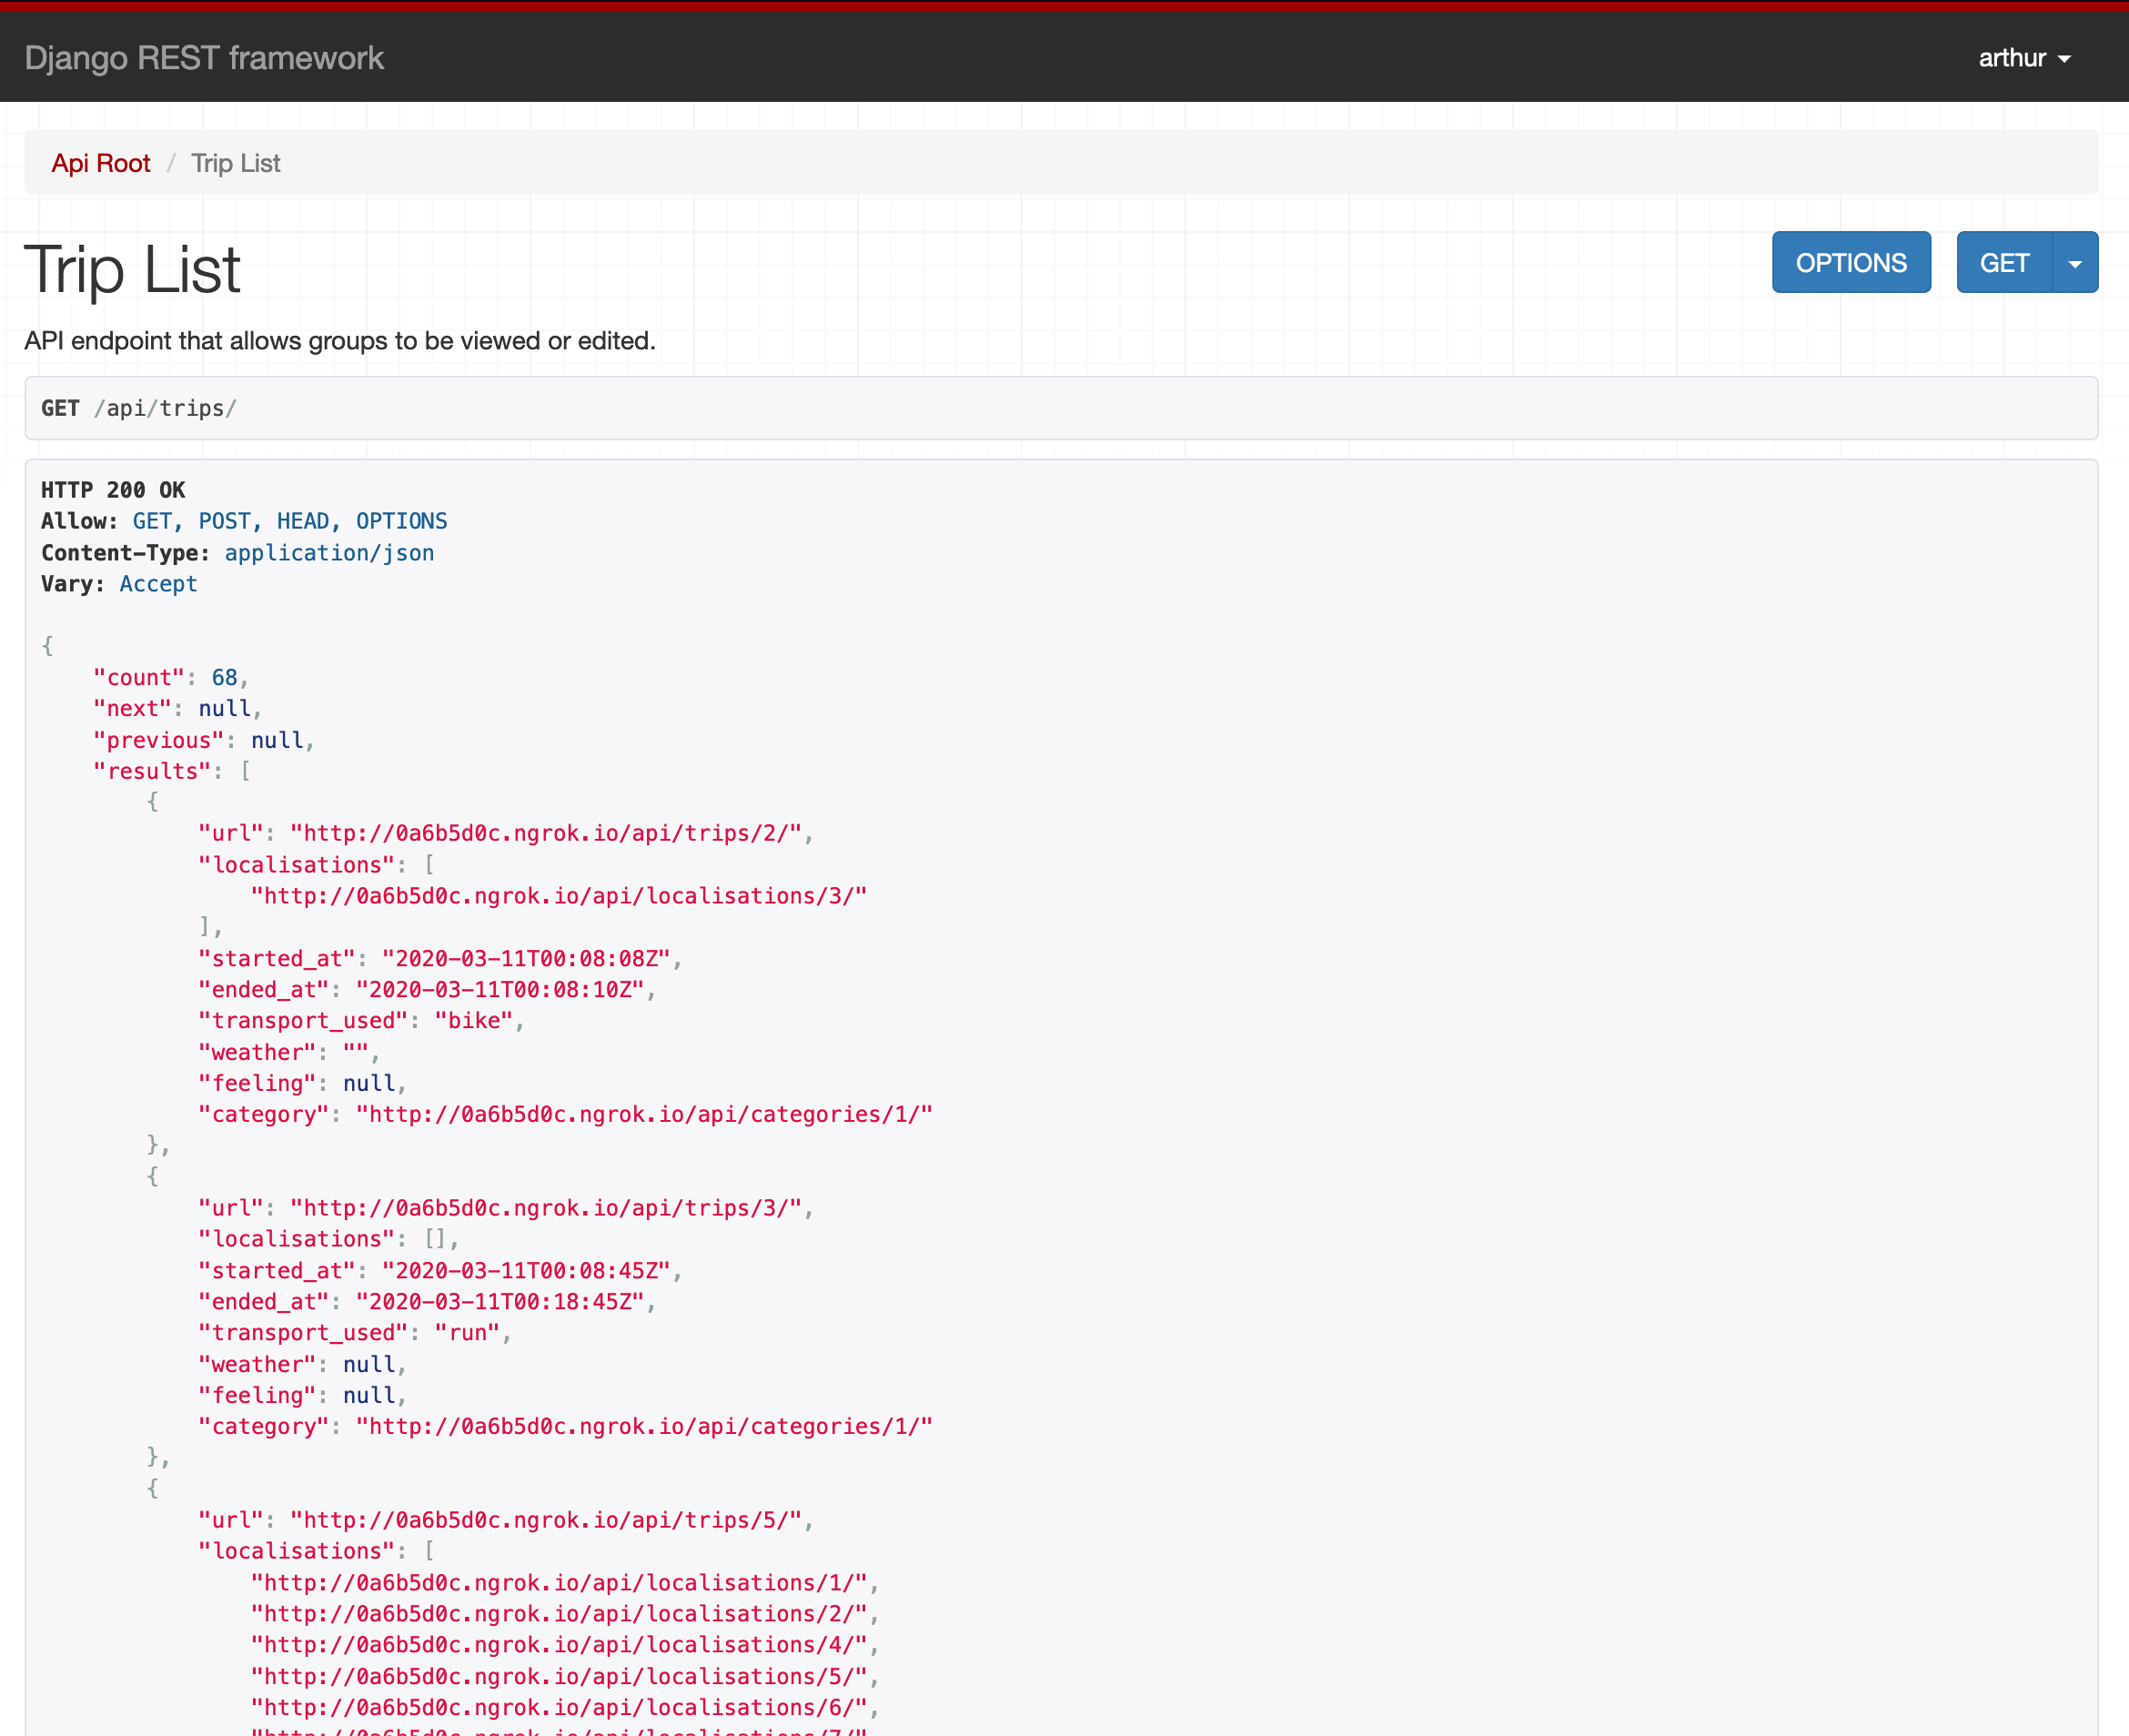
\includegraphics[keepaspectratio, width=2\textwidth/2, height=2\textheight/5]{ima/interface-api}
    \caption{L'interface de l'API utilisable pour le développement.}
    \label{fig:80-interface-API}
\end{figure}


\chapter{Manuel administrateur}


\section{Installation du site web}

Pour installer le site web, rien de plus simple. Tout d'abord, il vous faudra télécharge et installer python3.8+.

Sous Debian/Ubuntu,
\begin{verbatim}
    apt install python3
\end{verbatim}
devrait se charger de son installation automatiquement.

Ensuite, il faut utiliser pip pour installer les dépendances. Pour cela, déplacez vous dans le répertoire GhostRunWeb, puis lancez la commande suivante\footnote{Sur certains systèmes, la commande pip correspond a la version 2 de python ou n'existe pas. Dans ce cas, utilisez py -3 -m pip (sous windows) ou pip3, voire pip3.X, ou X est la version mineure de python.}

\begin{verbatim}
    pip install -U -r requirements.txt
\end{verbatim}

Une fois les requirements installés, vous pouvez lancer le site web. Pour cela, reportez vous à la section suivante pour une installation de développement, ou sur la section production pour une installation prête à être déployée.

\subsection{Pour le développement}

Lors du développement de l'application, il est plus simple d'utiliser une base de données SQLITE et le mode de débuggage de \Gls{django}.

Pour lancer le serveur, utilisez les commandes suivantes:
\begin{verbatim}
    # Crée la base de données sqlite et les tables correspondantes
    python3 manage.py migrate

    # Facultatif, mais permet la création d'un utilisateur
    # avec un compte permettant d'accéder à l'interface d'administration
    python3 manage.py createsuperuser

    # Lance le serveur sur le port 8000
    python3 manage.py runserver
\end{verbatim}

Le serveur est maintenant lancé et accepte les connexions. Rendez-vous sur \url{http://localhost:8000} pour utiliser le site web.

\subsection{Pour la production}

Pour le deployment, la base de données à privilégier est une base PostgreSQL. Son installation ne relève pas du domaine de ce document. Il est aussi nécéssaire de créer un utilisateur et une base propre à l'application.

Il faudra vous assurer que les données de configuration de production dans le fichier GhostRunWeb/GhostRunWeb/production.py sont correctes. Pensez à corriger les informations de connexion à la base de données, et l'URL du site web en production.

En vous aidant des instruction de la partie développement, vous pourrez créer les tables, et un superutilisateur.

Il est maintenant temps de rassembler les fichiers statiques pour qu'ils puissent êtres servis par le serveur web. Pour cela, utilisez,

\begin{verbatim}
    python3 manage.py collectstatic
\end{verbatim}

Pour lancer le serveur, il vous faudra un proxy, tel que nginx ou caddy, qui relaye les connexions depuis le port 80/443 (http/https) et sert les fichiers sur URL/static depuis le répertoire GhostRunWeb/static.

Une fois votre serveur web configuré\footnote{Une Caddyfile pour l'utilisation avec Caddy V2 est disponible en annexe}, lancez le site avec gunicorn (installé par pip), en utilisant les réglages de production.

\begin{verbatim}
    export DJANGO_SETTINGS_MODULE=GhostRunWeb.production
    gunicorn -b "127.0.0.1:8000" GhostRunWeb.wsgi -D --threads 8
\end{verbatim}

Si tout c'est bien passé, vous devriez pouvoir accéder à votre application à l'adresse configurée.

Pour finir, si vous utilisez Nginx, installez certbot pour obtenir un certificat vous permettant d'activer HTTPS sur le site.


\section{Compilation de l'application}

Pour compiler l'application, il est nécéssaire d'installer react-native (React Native CLI) sur votre ordinateur de développement. L'installation est documentée sur le site de react, à l'adresse \url{https://reactnative.dev/docs/environment-setup}, et varie grandement en fonction de l'OS utilisé.

\subsection{Pour le développement}

\subsection{Pour la production}


\section{Lancement des tests}

\subsection{Pour le site web}

Une fois le site web installé, les tests peuvent êtres lancés avec la commande suivante :


\begin{verbatim}
    python3 manage.py test
\end{verbatim}

Ces tests créent une base de données temporaire pour la session de tests qui sera détruite. Si l'un d'entre eux échoue, des "Falsifying example" peuvent êtres affichés : ils correspondent aux données qui ont amené le test à échouer.

Il est bon de noter que les tests peuvent facilement être lancés depuis PyCharm dans le cas ou le plugin \Gls{django} est installé et configuré.
